
% SIGMOD 2009 Submission
\documentclass{sig-alternate}
% the following package is added by mingxi
\usepackage {algorithm}
\usepackage {verbatim}
\usepackage {algorithmic}
\usepackage {times}

\usepackage {multirow}
\newtheorem{lem}{LEMMA}
\newtheorem{thm}{theorem}


\title{Joins in the DataPath Parallel Database System}

\numberofauthors{1}
\author{Horace Turnbuckle\\
horace$@$cise.unw.edu \\
University of New South Washington
             }


\newcommand{\todo}[1]{[\textbf{TODO: #1}]}
\newcommand{\eat}[1]{} % TO MAKE LARGE BLOCKS OF TEXT INVISIBLE
\newcommand{\sz}[1]{\lvert#1\rvert}
\newcommand{\card}[1]{\lvert#1\rvert}
\newcommand{\xp}[2]{P \if*#1\else^{#1}\fi \if*#2\else_{\! #2}\fi}
\newcommand{\pr}[3]{\xp{#1}{#2}\left\{\,#3\,\right\}}
\newcommand{\prl}[3]{\xp{#1}{#2}\{\,#3\,\}}
\renewcommand\:{\colon} % for use with \sset, etc.
\newcommand{\sset}[1]{\left\{\,#1\,\right\}}
\newcommand\xD{\mathcal{D}}
\newcommand\xP{\mathcal{P}}
\newcommand\xS{\mathcal{S}}
\newcommand\xbar{\bar x}
\newcommand\vbar{\bar v}
\newcommand{\eeblk}{\hbox{\lower 1pt \vbox{\hrule width6pt\hbox to
  6pt{\vrule height5pt depth1pt \hfil\vrule height5pt depth1pt} \hrule
  width6pt} \unskip}}
\newcommand{\eblk}{{\unskip\nobreak\hfil\penalty50
  \hskip1em\hbox{}\nobreak\hfil\eeblk
  \parfillskip=0pt\finalhyphendemerits=0\par}}
\newtheorem{xample}{Example}
\newenvironment{example}{\begin{xample}\em}{\eblk\end{xample}}
\makeatletter
\newenvironment{sql}%
 {\begin{list}{}{%
  \setlength{\topsep}{0pt}\setlength{\partopsep}{0pt}\setlength{\parskip}{0pt}%
  \setlength{\parsep}{0pt}\setlength{\labelwidth}{0pt}%
  \setlength{\rightmargin}{0pt}\setlength{\leftmargin}{0pt}%
  \setlength{\labelsep}{0pt}%
  \obeylines\@vobeyspaces\normalfont\ttfamily%
  \item[]}}
 {\end{list}\vskip5pt\noindent}
\makeatother

\def\email#1{{{\eaddfnt{#1}}}} % PJH: to fix weird bug in sig-alternate.cls

% END OF PETER'S MACROS

% BEGIN  OF ALIN'S MACROS

\newtheorem{defn}{Definition}
%\newtheorem{prop}{Proposition}
%\newtheorem{lem}{Lemma}
%\newtheorem{thm}{Theorem}

\newcommand{\pset}[1]{ \mathcal{P}(#1) }

%argument is the set; index is i, t not primed
\newcommand{\multsum}[1]{ \{ t_i \in R_i | i\in #1\} }
\newcommand{\multsumP}[1]{ \{ t_i^\prime \in R_i^\prime | i\in #1\} }
\newcommand{\multsumC}[1]{ \{ t_j \in R_j | j\in #1\} }
\newcommand{\multsumPC}[1]{ \{ t_j^\prime \in R_j | j\in #1\} }

\newcommand{\Set}[1]{ \{ 1\!:\!#1\}}

\newcommand{\E}[1]{ E\left[ #1 \right] }
\newcommand{\Var}[1]{ \sigma^2\left( #1 \right) }
\newcommand{\Cov}[2]{ \text{Cov}\left( #1,#2 \right) }


% END  OF ALIN'S MACROS



\begin{document}

\maketitle

%=========================================================================
%=========================================================================

\begin{abstract}
Blah Blah Blah Blah Blah Blah Blah Blah Blah Blah Blah Blah Blah Blah  
Blah Blah Blah Blah Blah Blah Blah Blah Blah Blah Blah Blah Blah Blah  
Blah Blah Blah Blah Blah Blah Blah Blah Blah Blah Blah Blah Blah Blah  
Blah Blah Blah Blah Blah Blah Blah Blah Blah Blah Blah Blah Blah Blah  
Blah Blah Blah Blah Blah Blah Blah Blah Blah Blah Blah Blah Blah Blah  
Blah Blah Blah Blah Blah Blah Blah Blah Blah Blah Blah Blah Blah Blah  
Blah Blah Blah Blah Blah Blah Blah Blah Blah Blah Blah Blah Blah Blah  
Blah Blah Blah Blah Blah Blah Blah Blah Blah Blah Blah Blah Blah Blah  
Blah Blah Blah Blah Blah Blah Blah Blah Blah Blah Blah Blah Blah Blah  
\end{abstract}

\section{Introduction}

The last five years have seen the design and development of an astonishing number of parallel databases, 
both research prototypes and industrial-strength systems \cite{}.  The designers of these systems have embraced the MPP 
or ``shared nothing''
approach, implicitly accepting the argument that the way to build a parallel database is to start with a number of
independent nodes---without shared memory or disk---and wire them together.
The advent of distributed batch processing systems such as Hadoop 
has only intensified the interest in large-scale, MPP systems. 

With all of the interest in building large-scale systems, the problem of building a shared-everything
parallel database to run
on one node has been mostly ignored over the last few years.  
We believe this is a critical error, for three reasons:

\begin{enumerate}

\item The individual nodes in a large-scale MPP system add more compute units and more RAM with every passing year.
A node that has 48 cores and
256GB of RAM can be purchased for around \$12,000 (excluding storage hardware)---this represents excellent value-for-money. Even if one asserts that
it is still more cost-effective to purchase less capable nodes, the fact is that with
every passing year, the inexpensive, commodity nodes in a distributed system will add more cores and more RAM.
The result is that increasingly, a large-scale MPP database system is really just a set of shared-everything 
parallel database systems networked together.
Thus, if one does not carefully consider how to build a parallel database
system that runs well on a single node, one is in 
danger of having a MPP system that scales out beautifully but can only
use a fraction of the compute power available to it.

\item For managing hundreds of terabytes of data, MPP is a necessity. But 
the number of consumers who actually need MPP is over-stated.
Good numbers are hard to come by, but
it is probably safe to assert that the median consumer of analytic database technology has tens of terabytes of data or less.
A \$12,000 machine with 100 billion machine cycles per second and I/O slots that support sustained 10GB/second
transfer rates should in theory suffice for managing ten terabytes of data.  Every hour, such a system can scan the entire ten terabytes 
3.5 times and expend 36 machine cycles per byte.  
Thus, most consumers (in theory) have little need for MPP and ideally should avoid it entirely, especially since distributed systems are
more difficult to build and maintain than a single node.

\item Tomorrow's 128 core machines will not be like the 128 CPU ``big-iron'' pushed by vendors 20 years ago. 
Thus, shared-everything database architecture needs updating.

\end{enumerate}

\vspace{5 pt}
\noindent
\noindent \textbf{The DataPath system.}
Taken together, these arguments make a strong case that shared-everything DBMS design is still a relevant problem.
Building a modern, shared-everything parallel database system 
is the goal of the DataPath project.  DataPath is  
designed to manage up to tens of terabytes of data on a single, inexpensive server machine.  It runs 
highly concurrent workloads ``out-of-the-box.'' It has no knobs to tune and runs on a single machine, 
so administration cost is negligible.  Yet it is still reasonably fast. Response times on ten terabytes 
of data are generally in the tens of minutes or less, even when many complex, ad-hoc queries are run 
simultaneously with one another.

Realizing that memory latency
and transfer bandwidth are the most severely constrained
resources in the target hardware,
DataPath attempts to achieve all of this by employing a ``data-centric'' approach.  
In DataPath, 
data flow in a relentless stream onto the system CPUs, where all operations that could use a piece 
of data process it simultaneously.  This tends to radically reduce data cache misses as well as I/O 
and memory bandwidth consumption, since computation is brought to the data, and not the other way around. 
DataPath is not the first system to employ a data-centric approach, but it is perhaps the most purely
data-centric system in existence, having been designed from the ground-up with the data-centric approach in mind.
An overview of DataPath has been published previously \cite{}.

\vspace{5 pt}
\noindent
\textbf{Joins in DataPath.}
This paper considers in detail one important aspect of the DataPath system: how the relational join 
operator might best
be implemented in a data-centric fashion.  Joins in database systems have been looked at extensively for 30 years, 
but DataPath's strategy resembles nothing we are aware of in an existing system, research or production.  
In almost every existing database system, joins are seen as isolated operations that have little or 
no interaction aside from indirect 
interactions resulting from competition for system resources.  And that competition can be very problematic;
it is not unheard of in commercial systems
for two queries running simultaneously to be slower than the same two queries running one after another.

This is not the case in DataPath. In-keeping with 
DataPath's data-centric approach, all queries use the same, monolithic hash table to process joins.  The hash table
and the data contained therein are shared by all.  Resource management is much easier because no particular query
owns the hash table, nor does a query own the resources needed to access the table.  The table itself ``decides'' when 
a query or queries are too expensive, and it evicts data from itself as needed, spilling it to disk in an orderly fashion.
Compared to the classical, compute-based paradigm where each operation owns its resources, it is almost trivial
for the central hash table to manage itself in a globally optimal way.

\vspace{5 pt}
\noindent
\textbf{Our Contributions.}
Our specific contributions are as follows.

\begin{itemize} 

\item We consider
join processing from an overall system design perspective, rather than as an isolated operation.
The system-based rationale for our various design choices is discussed carefully and in detail.

\item Join processing in DataPath is fast and efficient.
On a \$12,000 machine, during in-memory join processing DataPath can join nearly 300 million tuples per second.

\item As we show experimentally, on the same machine, DataPath can perform an external join of a multi-terabyte,
60 billion-row table with a multi-terabyte, 10 billion-row table in about 45 minutes.

\item In contrast to much work on parallel join processing, all of the algorithms we consider are explicitly multi-query aware.
All of our design decisions have been made with an eye towards simultaneously processing multiple large-scale join queries on a single
inexpensive machine.

\end{itemize}

\vspace{5 pt}
\noindent
\textbf{Paper Organization.}
Blah Blah Blah
Blah Blah Blah
Blah Blah Blah
Blah Blah Blah
Blah Blah Blah
Blah Blah Blah
Blah Blah Blah
Blah Blah Blah
Blah Blah Blah
Blah Blah Blah
Blah Blah Blah
Blah Blah Blah
Blah Blah Blah
Blah Blah Blah

\section{Joins In DataPath: Overview}

In this section, we give a brief overview of join processing in the DataPath system. 
Like all other aspects of DataPath, we strive to make join processing ``data-centric''.  What that means is that rather than
individual relational operations requesting data,
data are moved onto the CPU and all relevant computations---from all active queries---are 
performed on the data.  

In DataPath, all equi-joins are hash based. 
The most novel aspect of DataPath's join processing is that 
all equi-joins 
(even those from different queries)
share the \emph{same} in-memory hash table.  
All joins hash tuples to this table, and all joins probe this table to look for matches to tuples.
This hash is allocated when the system starts up, and takes up most of
the system's memory.  
In-keeping with the data-centric ideal, all tuples to be joined are ``owned'' by many queries.  When a tuple is
used to probe the hash table, all of its mates across all queries are accessed simultaneously.
Thus, the cache miss and memory transfer incurred by the probe are amortized across all queries using that tuple.

DataPath employs a single, monolithic hash table since
all tuples are shared by many queries---hence it makes little sense to partition tuples by query into different hash tables.
As we will discuss subsequently, there are many benefits to the ``monolithic table'' approach.
One key advantage is that there is no need to ever re-size a hash table to admit more data.  As we found during our
initial prototyping, using a dynamic-resizing approach (such as linear-hashing)
is exceedingly expensive in practice.  
Another advantage is that all join-related resource management and reclamation is centralized and
not run by any one query---this makes management and allocation of resources relatively simple.

When the central hash table becomes over-full, an entity called the \emph{cleaner} begins removing data 
from the hash.
The cleaner provides a natural mechanism for transitioning from an in-memory to a disk-based join.
Sometimes, the cleaner can reclaim enough space in the hash by removing stale data associated only with
queries that have completed. 
At other times, the cleaner determines that some active queries
are taking too much hash table space.  In this case, the cleaner ``wounds'' a group of queries, and begins streaming 
their tuples to disk; all wounded queries are in the process of
``switching over'' and becoming disk-based.  
Whenever the cleaner encounters a tuples associated with a wounded query, a copy of the tuple is removed from the
hash and written to disk.  
In this way, the choice of which 
queries are to remain in memory or moved to disk is made centrally, by the cleaner, based entirely upon the query's 
utilization of the central hash table.

Once a group of wounded queries have been fully cleaned from the hash and we are sure no other associated queries will
ever be hashed, completing the join is easy and efficient.
Since cleaning is performed in ascending order of the tuple's hash value, tuples that are removed from 
the hash and 
written back to disk are sorted according to their hash key.  Thus, once all of the tuples associated with a particular
join have been extracted from the hash and written to disk---at which point the query has moved from ``wounded'' to ``dead''---they
can be streamed off of disk
in ascending order of their hash key and then merged to complete the join.
In this way, DataPath naturally transitions from an in-memory, hash-based join to a disk-based, hash-merge join depending upon 
global resource availability. 

\section{Review of the DataPath System}

Before describing this process in more detail, we begin by giving the reader a high-level overview of query processing in general in the 
DataPath system.
This is a condensed version of the description from the original DataPath paper \cite{}.
Consider the following query:

\vspace{5 pt} \noindent $Q_1$: \begin{small} \texttt{SELECT SUM (l\_quantity)}\\
\noindent \texttt{FROM lineitem WHERE l\_shipdate > '1-1-06'} \end{small}

\vspace{5 pt} \noindent 
The DataPath system begins processing this query by starting a table scan of
\texttt{lineitem}. The system has just one circular table scan for
each table \cite{HarizopoulosSA05}.  All queries over a table share this scan.
Once the scan begins, tuples begin flowing along a ``path'' that leads out of the 
scan.  To allow $Q_1$ access to those tuples, DataPath creates a 
\texttt{selection} ``waypoint'' and attaches it to this path.
All work in DataPath is done by waypoints; waypoints are the only entities in the
system that are allowed to use significant CPU resources.  
Waypoint types include
\texttt{aggregate}, \texttt{join}, \texttt{groupBy}, etc.
The complete path network that is used to process $Q_1$ is 
depicted in Figure~\ref{fig:network}(a): it includes a \texttt{selection} waypoint, 
an \texttt{aggregate}, and a \texttt{print} waypoint that is tasked with outputting the
query result to the screen as the query completes.

Each waypoint has zero or more performance-critical routines that it runs in order to
process the data that are streaming through it.  For example, an \texttt{aggregate}
waypoint has a \texttt{ProcessMoreData} routine that aggregates some more data---adding tuples into a running
total in the case of a \texttt{SUM} aggregate---and a
\texttt{FinishUp} routine that computes a final aggregate once all of the
data for a query have been seen
A unique aspect of DataPath is that
all query-specific,
performance-critical code run by the waypoint is generated on-the-fly by the system, and then
compiled (using an off-the-shelf C++ compiler) when the waypoint
is created and/or updated with a new query. 

DataPath uses a token-based
system to dynamically allocate CPU threads to the various waypoints as the amount of
work that they wish to accomplish increases and decreases.
When there is actual work to do, a DataPath waypoint obtains a CPU token that gives it the right
to run the generated and compiled code on a thread.  A waypoint has no permanent storage other than
a small budget for meta-data that allows it to store its high-level state.  If it cannot obtain a CPU
token to process data that has been streamed into it, the data must be dropped and then re-produced 
and re-processed later.

\begin{figure} [t!]
\centering
\includegraphics[scale = .80]{IntroExample}
\vspace{-5 pt}
 \caption{An example path network in DataPath.}  
\vspace{-8 pt}
\label{fig:network}
\end{figure}

For performance reasons, DataPath does not move individual tuples through the network of waypoints.
All data are moved through DataPath as ``chunks of tuples''.
Chunks of tuples (or \emph{chunks} for short)
generally contain a large number of tuples (we use two million as the default size) so all fixed per-chunk costs
amortize to zero.  Each chunk is essentially an array of pointers to data columns, which are themselves contiguous arrays of
data with type-specific iterators.  Every column present in every query in the system
has one slot in the array of column pointers,
but most slots are unused in most chunks, since not all chunks contain all of the data
attributes in the system. Since all chunks are shared by all queries, very first slot
in the array of pointers
always points to the chunk's \emph{bitmap}, which records, for each of the queries present in the system, whether the query is
associated with the tuples in the chunk.  A \texttt{1} for the bit associated
with query $Q_k$ in the bitstring for the $j^{th}$ tuple in a chunk
means that the $j^{th}$ tuple is valid for
the $k^{th}$ query.  

In our example, now that $Q_1$ is up and 
running, imagine that the following two queries are issued:

\vspace{5 pt} \noindent $Q_2$: \begin{small} \texttt{SELECT SUM (l\_extendedprice)}\\
\noindent \texttt{FROM lineitem, order WHERE l\_shipmode <> 'rail'}\\
\noindent \texttt{AND o\_orderdate < '1-1-08' AND}\\
\noindent \texttt{l\_orderkey = o\_orderkey} \end{small}

\vspace{5 pt} \noindent $Q_3$: \begin{small} \texttt{SELECT AVG (l\_discount)}\\
\noindent \texttt{FROM lineitem, orders WHERE}\\
\noindent \texttt{o\_custkey = 1234 AND l\_orderkey = o\_orderkey} \end{small}

\vspace{5 pt} \noindent
When $Q_2$ is issued, a table scan of \texttt{orders} is begun and streamed into
into a new \texttt{selection} waypoint, but both $Q_1$ and $Q_2$ share all chunks
coming from \texttt{lineitem}.  To run the additional query, the code associated with the
\texttt{selection} waypoint attached to \texttt{lineitem} is re-generated,
re-compiled, and then injected into waypoint.
the This results in the path network of Figure~\ref{fig:network}(b).
Note that when chunks must be sent in two directions, only a shallow copy of the chunk is made; the actual data
contained in the columns is never copied.

Then, when $Q_3$ is issued, no additional waypoints are created; the system merely re-generates and re-compiles
the code associated with the relevant waypoints.  Note that in DataPath, two or more equi-joins may occupy the same \texttt{join} waypoint
as long as all of the equi-joins check for equality using exactly the same set of right-hand-side attributes.  
The result of adding $Q_3$ is Figure~\ref{fig:network}(c).

\section{Joins in DataPath: Design}

The three most distinguishing characteristics of DataPath's join-processing implementation are:

\begin{enumerate}

\item Equi-join processing in DataPath relies exclusively on hashing; sorting is not used.

\item All joins running in the system share the same monolithic hash table.

\item Rather than storing key-pointer pairs, all hashed records are stored directly in the hash table.

\end{enumerate}

In this section, we describe why we make these three choices.  In the next section, we will begin describing the technical
aspects of DataPath's join processing algorithms in detail.

\subsection{Hashing Or Sorting?}
This is the key question that must be answered when running any join.
In a traditional system, the answer might be: ``Have both available. Then at runtime
choose the one that is best for a particular query."

Unfortunately, deferring the question until runtime does not seem feasible given DataPath's data-centric approach.
In DataPath, no data object is ``owned'' by a query; instead, when a data object is processed, all interested
queries perform their computations over the data.
Allowing some queries to use sorting while some use hashing would require 
storing/organizing the data multiple ways during query processing, and
storing the data multiple ways depending upon the computational
requirements of the query workload is anathema to the data-centric approach.

One possibility would be to accept
that all queries inhabiting a waypoint must uniformly adopt a hash- or sort-based approach, and choose one or the other
on a per-waypoint basis.
The concern is that 
the first query to be added to a waypoint would force an ordering that is very poor for queries that 
are added later.  It seems best to choose a single organization that suffices for all queries, even if it is sub-optimal
for some.

\vspace{5 pt}
\noindent
\textbf{The Case For Hashing.}
If one accepts this line of reasoning, we need to choose either a sort-based or hash-based join. At
first glance, the hash-based solution seems 
preferable in a data-centric system, for the simple
reason is that it seems difficult or impossible to incrementally adjust sort-based data structures
to accommodate new queries that are added in an online fashion.
Let us make this argument concrete with an example.

Imagine that we have a query $Q_1$.  To process
$Q_1$, we begin streaming tuples relation \texttt{R} into a \texttt{join} waypoint so that they
can be sorted and 
joined with \texttt{S}.  After $Q_1$ begins execution,
query $Q_2$ enters the system; $Q_2$ also needs to sort \texttt{R} to join it with \texttt{S}.
$Q_2$ attaches to the table scan of \texttt{R}, the tuples being produced
by the table scan of \texttt{R} are marked as being attached to both queries, and those tuples are sent into a shared \texttt{join} waypoint.

After some time, all of the contents of \texttt{R} have been processed  
by $Q_1$, while $Q_2$ continues its execution.
Now, all of the tuples from \texttt{R} that have streamed into the \texttt{join} waypoint 
(some of which are associated with both $Q_1$ and $Q_2$) can be sorted
so they can be merged with tuples from \texttt{S}.  The question then becomes: what about the remaining tuples from \texttt{R}
that belong to $Q_2$, and continue to stream into the \texttt{join} waypoint? How are those processed?  
They could be buffered while $Q_1$ completes, but at some point the tuples
owned by both $Q_1$ and $Q_2$ must be merged with the tuples from $Q_2$ that continue to stream into
the waypoint.
This cost is linear in the size of the set of previously-sorted tuples, which seems prohibitively expensive, especially if the
number of tuples to be merged is small.
As an alternative,
one could move to some sort of staged, incremental sort (as epitomized by the LSM-Tree \cite{}),
but this would seriously
increase the complexity of the implementation, 
and it is unclear whether acceptable performance could be obtained.

This problem is non-existent in a hash-based solution.
One would simply hash all of the tuples from \texttt{R} that stream into the \texttt{join} waypoint; when the system is sure that all of
the tuples from \texttt{R} that belong to $Q_1$ have been added to the waypoint, the hash table is probed with tuples
from \texttt{S} that also belong to $Q_1$.  Concurrently, the remaining tuples for $Q_2$ can be added to the hash table.

\vspace{5 pt}
\noindent
\textbf{Cache Misses Revisited.}
This seems to argue strongly for a hash-based solution.  However, much research over the past 10-12 years argues that
hashing suffers from poor cache behavior, and some have even argued that a carefully-orchestrated sort-based join
is preferable (or will be soon) \cite{}.  
The problem is that performing a lookup in a very large
hash table incurs at least one random lookup and associated cache miss, and cache misses are phenomenally expensive in terms of CPU cycles lost in a
modern system.  
Does this not tip the balance in favor of sorting?

We do not think so.
One oft-overlooked fact is that sorting has its own cache
problems.  Given that sorting algorithms make multiple passes through the data, they can eat up significant
transfer bandwidth from RAM to CPU.
Thus, high-performance sorting algorithms (the best example of which is due to researchers from Intel \cite{}) sort key-pointer
pairs rather than full records---that is, 
the records are decomposed into key-data pairs, and the ``data'' part of the record is replaced with a smaller
pointer to the data to reduce bandwidth consumption.
Then, when the record is re-assembled, the pointer must be de-referenced, necessarily resulting in a random lookup.  
This results in one or even two random lookups per record output from a sort-based algorithm, which may actually be
\emph{worse} than a hash-based solution that hashes whole records.

\subsection{The Monolithic Hash Table}

As described previously, joins in DataPath are partitioned into
different \emph{waypoints}---the various joins making up a waypoint share the same left-hand-side input relation
and join attributes---this allows the hash table probe cost across all the queries in the waypoint to be amortized.  
Since queries can enter or leave the waypoint dynamically as they finish or start up their joins, there is no way to
know beforehand (or even to guess in any reasonable way) how much memory to allocate for a hash table associated with the waypoint.
This presents a difficulty for a hash-based approach because the hash table cannot be pre-sized appropriately;
sizing must be dynamic.

In our first prototype implementation, we decided to deal with this by using a linear-hash-based approach \cite{}.  Linear hashing re-sizes
a hash table dynamically by repeatedly doubling the table in response to insertions--when the table is doubled, a linear pass
through the table is made to re-hash all of the entries.
But after implementing such an approach we were astonished 
how slow loading data into the structure was, precisely
because of the re-sizing of the table.

The reason for the terrible performance required some investigation.
A key design goal of DataPath's hash-based approach is the ``one-random-lookup rule,'' which mandates that the 
the vast majority of hash table probes should incur only ony random memory access and associated expensive cache miss---see the next subsection for
a detailed discussion of this. A consequence of the one-random-lookup rule is that
``chaining'', where a linked list is hung off of an over-full hash table bucket to provide more space,
is not acceptable alternative in DataPath;
searching
a linked list necessarily incurs random lookups.  As a result, we use a simple linear scan to find empty space in the table, which
incurs no random lookups.
We did not anticipate how poorly this would work in conjunction with a linear-hash-based approach.
A table that is re-sized using linear hashing will usually have an area that is densely populated with data, having up to twice
the 
twice the density of the rest of the table.  This area
falls between the bucket that had last been re-hashed, and the first bucket in the ``new'' half of the hash table;
see Figure ???.  If one uses a linear-scan-based approach to deal with over-full buckets,
this dense area must some additional capacity, or the linear scan will be unable to find storage in this region
for data from an 
over-full bucket.  Since this dense area can be twice as dense as the rest of the hash table,
a maximum fill factor of at most 50\% for the overall table should be used.  

\begin{figure}[t]

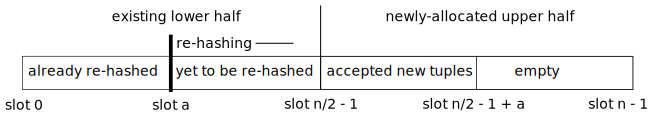
\includegraphics[scale=0.47, angle = -90]{Rehashing.pdf}
\caption{Illustration of a linear hash table.  The region between slot $a$ and slot $n/2 - 1$ can have as much as
twice the density of the rest of the table.}

\end{figure}

Given a maximum fill factor of 50\%, to add $N$ bytes of data to the hash table, 
at least $8N$ bytes of data must be read/written, which is exceedingly expensive.
Where does the $8N$ figure come from?  Ignoring momentarily the cost of re-sizing the table, writing $N$ bytes of data to a hash
table requires reading approximately $N$ bytes (each bucket must be transferred onto the CPU so the new record can be written to it), and
then writing $N$ bytes out to RAM.  Also, the total number of bytes 
transferred while incrementally re-sizing a linear hash table to reach size $M$ is 
$M + M + \frac{M}{2} + \frac{M}{4} + \frac{M}{8} + ... = 3M$.
This expression reflects the fact that 
each byte in the table must be written when it is re-hashed into, whereas half must be re-hashed at least
once (at a cost of an additional read and
a write, past the initial write), a quarter must be re-hashed at least twice (at the cost of two additional reads and writes, past
the initial write), an eighth must be re-hashed at least three times, and so on.  If $M \geq 2N$ to ensure that the dense section of the
table does not interfere with the linear scan, then the overall cost in terms of RAM transfer is at least $8N = 2N + (2 \times 3N)$.
This is far too high.

Facing such an unpalatable alternative, we decided to do the obvious thing: we use a hash table that is so large it need never be re-sized,
because it uses all of the system RAM.  By definition, such a table must be shared across all joins, because
the table uses almost all of the
system RAM.  Adding $N$ bytes of data to such a table requires only $2N$ bytes of memory bandwidth, a quarter of the bandwidth
consumed by the linear-hash-based approach.  

\subsection{The One-Cache-Miss Rule}

The last design goal we discuss is our self-imposed ``one-random-lookup rule'', 
which requires that the typical hash table probe in DataPath incur one and only one random lookup and associated expensive cache miss.

It has long been recognized that CPU cache misses are phenomenally costly in database systems, particularly
when running hash-based joins, since accessing a random slot in a hash table can be expected to result in a cache miss \cite{}.
In response, a large number of 
special ``cache-conscious'' join algorithms---sometimes closely tied to specific hardware---have been proposed.
Our own experimentation and analysis shows that yes, cache misses are expensive, but that they are not expensive enough
to require special algorithms that pre-fetch hash table slots or that ensure that the hash table fits in L2 CPU cache.
Instead, we accept one and only one random lookup per hash table probe, and do everything we can to ensure that 
additional random lookups are not incurred; practically speaking this means requiring that 

How expensive are random lookups?  A simple C program running on the \$12,000 machine described in the introduction
serves as a good micro-benchmark.  
In a loop, the program repeatedly uses an 
inline random number generating algorithm to select and access
a random integer from an array, which is added
into a running total.  
If the array is sized so that it fits entirely in L1 cache (so there are no cache misses due to random lookups) the program is able to perform 
69 million additions per second, for a total of 14 nanoseconds per addition.  If the array is sized so that it fits in L2 cache, then
this drops to 22 million additions per second, or 45 nanoseconds per addition.  
If the array is made very large so that every access results
in a fetch from RAM, this drops to 10 million additions per second, or 100 nanoseconds per addition.

Thus, we are experiencing a hit of 86 nanoseconds (compared to ``perfect'' cache behavior), or about 200 instructions lost, worst case.
Let us put this in perspective: our \$12,000, 48-core machine can---in the best case---can run around 200 billion
instructions per second, and---in the best case---load around
100 million, 96B records from disk and into RAM per second.  This means that the system
can suffer approximately $10 \approx \frac{2 \times 10^{11}}{200 \times 10^8}$ cache misses due to random lookups
per 96B record before it is CPU-bottlenecked, or
around three random lookups per 24B record.  
Granted, system CPUs will be doing other work besides hash table lookups, so not all of those cycles are available to wait on a memory
transfer.  But not every record will be joined multiple times, either; many will be filtered by selections,   
or be part of a query that does not have a join.
Thus, cache misses are precious, but not overly so---hence the one-random-lookup rule.

\section{Hash Table Basics}

Having established that hashing is the preferred alternative, and that we will use a single, monolithic table,
we describe in detail how tuples are added to the monolithic hash table during join processing, and how 
the table is probed.
Our algorithms as well as the low-level details of the hash table design are dominated by two requirements:

\begin{enumerate} 

\item
The one-random-lookup rule.
As dictated by this rule, an \emph{entire} tuple to be joined must be written to the hash
table and not just the join key, no matter
the size of the tuple.
In this way, a second
random lookup associated with accessing the non-key part of the tuple is avoided when the table is probed.

\item 
Efficient concurrency control. Readers should have to obtain no locks to read, and the number of per-tuple locks obtained
by a writer, amortized over the number of tuples hashed, should be nearly zero.
\end{enumerate}

\subsection{Overview}

Given these requirements, our design is as follows.
When a chunk enters a \texttt{join} waypoint, it is either a ``left-hand-side join chunk'' (``LHS chunk'' for short)
or ``right-hand-side join chunk'' (``RHS chunk'' for short).  Assuming that
the waypoint is running an in-memory (not disk-based) join, 
a RHS chunk is always broken into tuples and then stored in the monolithic hash table, and
a LHS chunk is used to probe the hash table and look for matches; in an in-memory join, all tuples from all RHS chunks are added to
the hash table before any LHS chunk is sent to the corresponding waypoint.

\begin{figure}
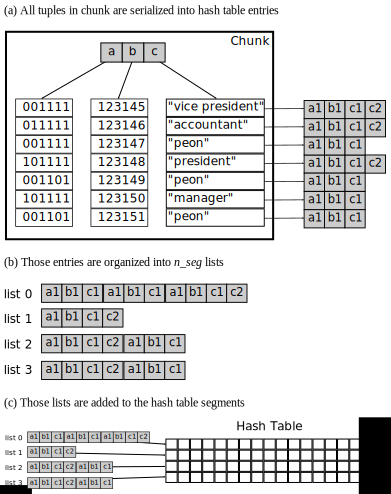
\includegraphics[scale=0.75]{Serialization.pdf}
\caption{The process of adding a chunk to a hash table.} \label{serialization}
\end{figure}

When a RHS chunk enters a \texttt{join} waypoint, the following steps are undertaken:

\begin{enumerate}

\item 
Tuples in a chunk
are stored column-wise, in a list of arrays, where each array stores all of the values for all of the tuples
for a particular
attribute.  The
first step in adding the tuples to the hash
table is to transform them to a row-oriented format so they can be stored in the hash table.
This process is referred to as ``serialization.''

\item
As the tuples are serialized,  we partition them into a set of
$n_{seg}$ lists, so that all of the tuples that are going to be written 
to the same region of the hash table are co-located in the same list.
A tuple $t$ is appended to list $i$ if
$h(t) \textrm{ }\texttt{mod}\textrm{ } n_{seg} = i$, 
where $h(t)$ denotes the hash value of the tuple. 
$n_{seg}$ is the number of \emph{hash table segments},
where a hash table segment is a distinct region of the hash table; all of the tuples with the
same $h(t) \textrm{ }\texttt{mod}\textrm{ } n_{seg}$ will be written to the same hash table segment.
As we describe below, the key reason for breaking the hash table into segments is concurrency control: 
writers will lock the hash table at the segment level.
Note that even though multiple queries may be utilizing $t$, as was described in Section 3,
to be together in the same join
waypoint, they must all be performing an equality check using the same attributes from $t$, and so $h(t)$ will
be the same accross all queries.

\item
Finally, the $n_{seg}$ lists are added to the hash table.  To do this, the system
randomly selects a hash table segment that does not currently have a writer.  
Each hash table segment can have at most one writer, and an arbitrary number of concurrent readers.  
If segment $i$ is selected, then a single, linear
pass is made through list $i$ and all of the tuples 
that have been serialized to list $i$ are hashed to segment $i$.
Assuming that there are $n_{slot}$ entries in each hash table segment, a tuple $t$ in list $i$ is 
added to slot $(h(t) \textrm{ }\texttt{mod}\textrm{ } n_{seg} \times n_{slot}) \textrm{ }\texttt{div}\textrm{ } n_{seg}$ in the $i$th hash table segment.
This step is repeated for each of the $n_{seg}$ lists.  If, at any time, there is no $i$ for which (a) list $i$ has not yet been
hashed, and (b) segment $i$ is not currently being written by another hasher, then the thread hashing the
RHS chunk blocks until such an $i$ exists.

\end{enumerate}

The process of serializing a chunk and writing it to the monolithic hash table is depicted above in Figure \ref{serialization}.

\subsection{Serialization In Detail}

This subsection describes in detail how tuples are serialized.

In DataPath, each hash table segment is a simple array of twelve byte
hash table entries; each entry consists of four bytes of metadata, and eight bytes of
data.  Tuples that are inserted into the hash table are written to this array, and so 
the ``serialization'' of a tuple
refers to the process of taking a tuple and writing it to a sequence of hash table entries that can then be copied
into the hash table.

Because a serialized record can be of arbitrary size, it can be written to an arbitrary number of hash table entries.  
For example, reconsider Figure \ref{seriaization}. The first attribute, attribute ``a'', is the query-membership
bitmap, and happens to be eight bytes
or less.  So it is serialized to a single entry labeled ``a1.''  Likewise the attribute ``b''.  But the third attribute ``c'', which
is a string, is variable-length and may take up two hash table entries.  By 
convention, bytes from different attributes in the same tuple are always written to different entries, even if 
they could be packed together in the same entry---this makes it easier to de-serialize the tuples later on---though 
larger attribute values may span multiple entries.

In
DataPath, there are two types of hash table entries: \emph{start entries} and a \emph{continuation entries}.  As the names suggest, a
start entry marks the start of a serialized tuple and will always contain the tuple's bitmap,
and an continuation entry is any entry devoted to storing any other attribute from the tuple.

The metadata for both types of hash table entries begins with the following information:

\begin{enumerate}

\item A bit that indicates whether the entry is used.

\item A bit that indicates the type of the entry (start or continuation).

\item The distance (in number of hash table entries) to the next entry containing data associated with this tuple.
If an entry is written to slot $s$ in the hash table,
we will subsequently refer to this value as the ``offset for slot $s$''.

\end{enumerate}

In the case of a start record, the metadata also contains the distance (that is, the number of hash table 
entries) from the hash table slot that the start entry 
for the tuple \emph{should} have been written to, were there no collisions.
We will subsequently refer to this value as the ``distance from the true position'' for the tuple.

Finally, the start record contains a unique identifier associated with the waypoint that the tuple belongs to,
as well as a bit that indicates if this is a record from a LHS chunk or a RHS chunk.  While in-memory joins write only
RHS chunks to the table, as we will see shortly, if
a join adds too much RHS data to the table, it is ``wounded'' and becomes disk-based.  In this case, the join will
write LHS chunks to the table as well.

In the case of a continuation entry, the metadata also contains an identifier indicating which attribute in the tuple
the eight data bytes are associated with.

\subsection{Writing to the Table}

Once all of the tuples in a chunk have been serialized to one of the $n_{ent}$ lists, those
lists are processed one-at-a-time, and all of the serialized tuples contained in each list are written to the same
hash table segment.
 
When a serialized tuple $t$ that has been assigned to a hash table segment is to be written
to that segment, we first check to see if the entry at slot 
$h(t) \textrm{ }\texttt{mod}\textrm{ }n_{ent}$ is occupied.  If it is, then a linear, forward scan in the hash table
is performed until an empty entry is found---we'll assume this is slot $s$.  
At this point, a start entry containing $t$'s bitmap is written.  In
addition, the value $s - h(t) \textrm{ }\texttt{mod}\textrm{ }n_{ent}$ is written to the entry as the ``distance from the
ture position'' for the underlying tuple, so a query
will know where the tuple should have been in the hash table, and
will not be forced to de-serialize and check tuples that cannot possibly match.

Enough space is allocated in the four bytes of meta-data associated with a hash table entry to store an offset of
2048 slots.  If there are an excessive number of collisions or a significant amount of skew, the actual offset may
exceed this number.  In that relatively rare case, the offset is stored in a lookup table external 
to the hash.

Once the bitmap has been written, the remainder of the hash table entries making up the tuple are written.  
Beginning at slot $s$, a linear scan is performed to find the first unused entry in the hash table; we'll call this
slot $s'$.  The first entry associated with the first non-bitmap attribute is then written to the entry
at slot $s'$; in addition, the offset for slot $s$ is set to $s' - s$,
so that queries finding the tuple can hop among the entries that make up $t$.

\begin{figure}
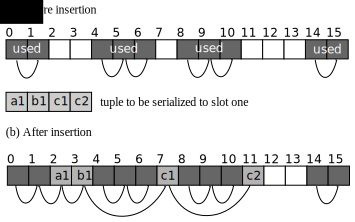
\includegraphics[scale=0.85, angle=-90]{AddingToTable.pdf}
\caption{Writing a serialized tuple to the table. After the tuple is written,
the start entry (a1) has a ``distance from its true position'' of one, and all entries have offsets indicating where
the next entry in the tuple is found; for example, the offset associated with c1 is four.} \label{writingtuple}
\end{figure}

This process is then repeated for each of the entries that make up the tuple.  Beginning at the last slot written, a
linear search is employed to find the first unused entry.  
The next eight bytes are written to that entry, and then the appropriate offset is written to the previous entry.
This is depicted above in Figure \ref{writingtuple}.

\subsection{Hash Table Probes}

Once a query's RHS input relation has been fully hashed, DataPath begins streaming the LHS input relation into
the \texttt{join} waypoint to complete the join.
When a LHS chunk enters a \texttt{join} waypoint, each of the tuples contained therein are used
to probe the hash table and look for potential RHS mates.
The process of finding all of the mates for a LHS tuple $t$ is as follows:

\begin{enumerate}

\item First, the LHS tuple $t$'s join key is hashed to obtain the identity of the segment $i = h(t) \textrm{ }\texttt{mod}\textrm{ } n_{seg}$ and the slot 
$s_0$ $=$ $(h(t)$ $\texttt{mod}\textrm{ } n_{seg}$ $\times$ $n_{slot})$ $\texttt{div}\textrm{ } n_{seg}$
where a potential mate might be found.

\item The value $s$---which is the current slot we are probing---is initialized to $s_0$.

\item The hash table entry at slot $s$ in segment $i$ is checked to see if it may possibly be a match for $t$.  There are three cases.

\begin{enumerate} 

\item The entry is not used.  In this case, we are done with $t$, since there is no way that the insertion algorithm would have
skipped over an empty slot at position $s$ to write a RHS mate for $t$ into the hash table.

\item The hash table entry is used, but it is not a start entry.  In this case, we happen
to have hit the middle of a tuple.  This cannot possibly be a match for $t$, because $t$ must have started at or after slot $s$.
So we let $s = s$ $+$ $($the offset for slot $s)$, and repeat from step (3).
If the offset for slot $s$ is zero (which signifies that the entry at slot $s$ ends a tuple), then $s$ is incremented by one.

\item The hash table entry is used, and it is a start entry.  In this case, we check to see if this is a potential match 
by verifying that both (a) the tuple with start entry at slot $s$ comes from the same waypoint as $t$, and (b) 
the distance from the true position of this tuple is $(s - s_0)$---this verifies that the tuple we have found in the hash
table hashed to the same position as $t$.  If either of these do \emph{not} hold, then we have 
not found a potential mate and we update $s$ exactly as in (b) above, and then we repeat from step (3).

\end{enumerate} 

\item If we have made it here, then we have potential mate.  So we de-serialize the tuple
we have found by following the chain of linked hash table
entries starting at slot $s$, incrementing $s$ as we go, exactly s described under step (3b).

\item Once we have de-serialized the potential RHS mate, we can then check
to see if it joins with $t$.

\item Finally, we repeat the process again, starting at step (3).
\end{enumerate} 
 
\vspace{5 pt}
\noindent
\textbf{Optimized Probing for Foreign Key Joins.}
There is an important performance optimization that DataPath utilizes when it is probing the hash table.  As we
have asserted repeatedly, memory
bandwidth and access are the most precious resources available to the system, and constructing an entirely
new chunk to output from the join can be exceedingly expensive in this regard, particularly considering the bandwidth
required to copy copious amounts of LHS data to the output chunk.  

This can be optimized in the very common case where the join is acting as a filter for the tuples in the LHS
chunks---that is, for the case where there is zero or one copy of each of the LHS tuples in the chunk output from the join.  
This is the case, for
example, when the underlying joins are all foreign key joins of the LHS into the RHS.

The optimization works as follows.  Initially, all of the columns that come from the LHS chunk are copied into the
output chunk using only a shallow copy. As the LHS tuples are used to probe the hash table, the only columns that
are updated are (a) the bitmap column where \texttt{1} bits are flipped to \texttt{0} in the case that
a match is not found, (b) any columns that come from RHS tuples stored in the hash table, 
and (c) any columns that are ``synthesized''---that is, columns whose values are created by applying some function to 
RHS or both LHS and RHS tuples.  Often, no columns at all fall into categories (b) and (c), so the only column being
updated is the bitmap, which is inexpensive.

This goes on until the first LHS tuple is found that has more than one RHS mate.  Often, this will never happen and
the shallow copy will be sufficient.  In the case that some LHS tuple is found to have more than one mate, the shallow copy no
longer suffices because the number of tuples has changed.  In this case, the join becomes more expensive and deep copies of all 
all of the LHS columns are added to the output chunk.  Probing then resumes,
except that now, all columns are written as additional tuples are processed.

\subsection{Concurrency}

Of course, it is crucial that readers (performing LHS probes) 
and writers (performing RHS hashing) both be able to access the central hash table concurrently without any significant
performance penalty for doing so.  

Concurency control during hashing is exceedingly simple.
Under our scheme, a writer first breaks the chunk to be hashed into a set of 
lists, with one list per segment, locks the segments one-at-a-time, and adds all of the tuples in the list associated
with that segment while it is locked.
Thus, the total number of locks obtained by a writer to hash all of the tuples in a chunk is $n_{seg}$; since $n_{seg}$
is orders of magnitude smaller than the size of a chunk, the cost associated with concurrency control amortizes down to zero.
Readers need not obtain any locks at all.

\vspace{5 pt}
\noindent
\textbf{Correctness.}
Under this scheme, writer-writer and reader-reader conflicts are clearly not possible: writers cannot be in conflict
because they must lock segments, and readers cannot be in conflict because they do not update anything.  

It is perhaps more surprising
that this simple scheme avoids reader-writer conflicts without requiring that readers actually lock anything.
It is true that multiple readers can be probing a segment that is being written.  But since each individual join is either
probing or hashing---a join cannot begin probing until its RHS has been fully hashed---a writer inside of a segment must be
writing tuples associated with a set of queries that is distinct from the set associated with every reader in the segment.
Thus, the only concern is that the presence of the writer may disrupt a reader, by writing only a portion of a serialized
tuple that the reader then accesses.  This is not a problem, either.  The mere fact that the writer is writing to a hash
table slot indicates that the slot was empty previously, which in turn means that the reader could stop looking for a mate
at that point.  Finding a half-written tuple is not problematic.
As long as the writer first writes the eight bytes of data to the hash table entry and then writes the
four bytes of meta-data, and the latter write is atomic (as it will be on virtually all hardware), 
the reader will first find that the slot is used, and then---if the partially-written tuple happens to have the same hash key and it happens to 
come from the same waypoint---the reader will de-serialize as much of the tuple as has been written.  
After deserialization, the reader will check the bitmap (which is valid)
to see if the partially-written tuple is associated with the same query or
queries as the probe, which it cannot be.  The the reader will ignore the rest of the partially-written tuple,
and no harm is done.

\vspace{5 pt}
\noindent
\textbf{Choosing the number of segments.}
$n_{seg}$ is a constant chosen with two considerations in mind.  First, it should be large enough so that all of the threads
adding data to the hash table can have their own segment locked.  As described in Section 3,
DataPath uses a token-based scheme where waypoints request CPU
tokens that allow them to schedule computationally-expensive operations, such as hashing.  A good rule-of-thumb is that $n_{seg}$
should be larger than the number of CPU tokens.  This ensures that even if all of the system CPU resources are being used to hash tuples,
as long as the various CPUs are being used to hash to different segments, no writer will be waiting on a hash table segment.
At the same time, $n_{seg}$ should be small enough
that the tail of each of the $n_{seg}$ lists can fit in L1 cache simultaneously; that way, there are no random memory accesses 
incurred during serialization and all memory transfers are fully sequential. We use $n_{seg} = 128$ in our 
prototype implementation, which runs on a 48-core machine.  

\section{The Cleaner}

Everything described thus far assumes that the space in the monolithic hash table is limitless, and that it never fills.
Of course, this is not the case.  It is the responsibility of a software component called 
the \emph{cleaner} to ensure that there is always enough
space to write new data into the hash.

The cleaner has two related responsibilities:

\begin{enumerate}

\item Removing data associated with completed queries from the hash.

\item Removing data associated with \emph{wounded} and \emph{dead}
\texttt{join} waypoints from the hash.  Wounded and dead waypoints have become
disk-based.  A waypoint is said to be \emph{wounded} when the cleaner has determined
that it is taking up to much space in the hash table.  When the cleaner wounds a waypoint, no new queries
are attached to the waypoint, and \emph{both} the waypoint's LHS and RHS chunks are added to the monolithic
hash table.  The cleaner will spill both LHS and RHS data associated with a wounded waypoint to disk for subsequent processing.
Once wounded waypoint has added all of its LHS and RHS data to the hash, it is said to be \emph{dead}---at this point,
the waypoint can be removed from the system.

\end{enumerate}

\subsection{Invoking the Cleaner}

Whenever new data are added into a hash table segment by a \texttt{join} waypoint, a small number of random probes are performed on the segment.
These ``sample'' probes are used to see how full the segment is.  If a fraction greater than the
``hard cap'' $l_{hard}$ of these probes hit slots that
are used ($l_{hard} = 0.7$ in our implementation), then the segment is declared to be over-full,
and the contents of those slots are turned over to the cleaner 
for processing, along with a request that the segment be cleaned.

When the cleaner receives those sampled slots, it first looks at the status of each of the \texttt{join} waypoints and queries that were sampled
to determine how it can reduce the fill factor so that it is at most $l_{soft}$, where $l_{hard} > l_{soft}$.
Sometimes, it will be possible to achieve this by simply removing data from the segment that is already slated for removal.
There are two types of data that are always removed from a segment:

\begin{enumerate}

\item
Data in slots that are associated only with queries that are complete.

\item Data in slots that were written by dead or dying waypoints.

\end{enumerate}

\begin{figure}
\includegraphics[scale=0.5, angle=-90]{Augmented.pdf}
\caption{A path network augmented with the additional waypoints needed to support disk-based joins..} \label{augmented}
\end{figure}

When a RHS chunk enters a \texttt{join} waypoint, the following steps are undertaken:

If the cleaner looks at the sampled slots and determines that it cannot get the fill factor down to $l_{soft}$ by removing such data, it 
must wound one or more active \texttt{join} waypoints, thereby declaring them to be disk-based, and slating their data for removal from the segment.
Our current implementation chooses waypoints to wound in a rather simplistic, greedy fashion, by choosing to wound the waypoint taking up the most space
in the table, and then the waypoint with the second most space, and so on, until the fill factor is reduced sufficiently.
An obvious improvement to this would be to take into account the extent to which the query has completed---for example, we might be more
hesitant to wound a waypoint which has fully hashed the RHS data for all of its queries.  This would make sense because we know that
the amount of space that the waypoint takes up in the hash table is not growing and that its queries are in the process of finishing up.
Designing a better scheme is a problem left to future work.

\subsection{Operation}

Once the cleaner has determined that one or more segments need to be cleaned and how to clean them, it requests the CPU tokens it needs to
begin its work.  One CPU token (and hence one thread) is used to clean each segment.  

When cleaning a segment, the cleaner first obtains a write lock on the segment.  
Readers can continue to probe the segment during cleaning.
The cleaner then allocates enough space to hold a new version of the segment, and 
makes a linear pass through the segment to be cleaned, from low hash value to high hash value.  
If the cleaner finds a tuple from a completed query, the cleaner ignores the tuple.
If the cleaner finds a tuple from a query that has not finished from a waypoint that is neither dead nor wounded, a copy of the tuple
is moved into the new segment.  

The interesting case is when the cleaner finds a tuple from a dead or wounded waypoint that is associated
with a non-completed query.  As the cleaner cleans a segment, it constructs two chunks per dead and dying waypoint.  One of those chunks
holds LHS tuples, and one of those chunks holds RHS tuples.  When the cleaner encounters a tuple from a dead or dying waypoint, it uses
the start entry's meta-data to determine if the tuple is a LHS tuple or a RHS tuple; the tuple is then appended to the LHS or to the RHS
chunk associated with the dead/dying waypoint.  Since the cleaner works its way through the hash table segment sequentially, all of the tuples
are written to the ``extraction chunks'' in sorted order of their hash key.

When the cleaner finishes cleaning a segment, it then sends each of the extraction chunks to a set of \texttt{joinIO} waypoints.
There is always one \texttt{joinIO} waypoint for each of the \texttt{join} waypoints in the system---not surprisingly,
the \texttt{joinIO} waypoint reads/writes data to/from disk on behalf of a \texttt{join} waypoint.
If a waypoint is never wounded, its associated \texttt{joinIO} waypoint will never be used.
But once it is wounded, data associated with the waypoint must be spilled to disk.  The \texttt{joinIO} waypoint is used to write to disk the 
chunks associated with a wounded waypoint, and, later one when the waypoint is dead, the assocaited \texttt{joinIO} waypoint will begin
re-reading those chunks from disk so that they can be joined.
As an example, a path network 
that has been agumented with the necessary \texttt{joinIO} waypoints is depicted above in Figure \ref{augmented}.
Note that there is one \texttt{joinIO} waypoint per \texttt{join} waypoint.
The \texttt{merger} waypoints that also appear in this figure will be described subsequently.

When a \texttt{joinIO} waypoint receives a chunk from the cleaner, it must either acknowledge it and write a copy to disk, or drop it.
Drops can occur when there is not enough disk bandwidth available to write all of the 
extraction chunks at the sepeed
they are produced.  
At the first drop,
the cleaner de-allocates the new version of the segment that it has constructed.
The cleaner batches all of the drop messages it receives as a result of cleaning a segment.  
Once all of the
extraction chunks it created have been dropped or acked, the cleaner 
either swaps the new version of the segment into the hash table, deallocating
the old one and finishing the cleaning of the segment (this is done if none of the extraction chunks were dropped), 
or else it re-creates the new segment as well as any dropped
extraction chunks and re-sends the recreated extraction chunks to the relevant \texttt{joinIO} waypoints.  
The new segment is re-created and the extraction chunks re-sent as long as at least one extraction chunk has been dropped.

The reader may question why we decided to re-clean the segment and re-create dropped chunks, rather than
saving the chunks and trying again.  
The reason is simple: chunks are meant to be an ephemeral mechanism for streaming tuples onto or off of a CPU, 
as opposed to being used as storage containers.
Almost all system RAM is consumed by the monolithic hash table, and so there is simply not enough RAM to have a large number of buffered chunks
sitting around.  

\section{External Merges}

When a wounded waypoint has finally hashed all of its LHS and RHS data, it is ``dead''.  Once the waypoint dies and the cleaner makes one
complete pss through the hash table, cleaning all of its segments, we can be sure that all of the waypoint's data has been written to disk.
At this point, the \texttt{joinIO} waypoint associated with the
dead \texttt{join} waypoint stops writing data to disk, and begins reading it.  The \texttt{joinIO} waypoint chooses
a segment $i$, and then re-reads all of the chunks it wrote that are associated with segment $i$.  Those chunks are bundled together, and sent
to the associated \texttt{merge} waypoint.  This is done for each
segment; once all segments have been merged, the dead \texttt{join} waypoint has completed and it can be removed from the path network.

Because the cleaner created the various chunks by sequentially cleaning the segment, the tuples contained therein are already
sorted on the hash key.  So to completely join all of the tuples from segment $i$, a simple merge is used, where each of the extrction chunks
are scanned from front to back.  All of the discovered output tuples are appended to an output chunk, which is then sent on to the waypoint
that would have received the output of the original \texttt{join} waypoint, had it never been wounded in the first place.

One issue that deserves a bit of explanation is how to deal with joins of very, very large database tables.  As described thus far, we implicitly 
assume that we have enough memory to store all of the chunks ever extracted from segement $i$ in main memory, so they can be merged.  
This is an unreasonable assumption.  

To handle this, the cleaner inserts a set of \emph{markers} into the columns
that make up the extraction
chunks, as they are created.  We use $128$ markers in our implementation.
Each marker is associated with a hash key value, so that (for example)
to read only those tuples having hash keys in the first $\frac{1}{128}$ of an extraction
chunk, the \texttt{joinIO} waypoint need only read to the first marker.  To keep memory consumption reasonable, the \texttt{joinIO} waypoint can use
these markers to avoid processing 
the whole segment at once.  It can use the markers to break the segment up, thereby merging all of the data in the segment in a series
of smaller merges as opposed to one very large merge.

One final issue that is worth discussing is the actual implementation of the merge.  When merging all of the chunks from segment $i$, it is necessary
to have a priority queue that is used to find the tuples
with the lowest (smallest) hash key value in all of the LHS chunks that has not yet been processed, 
as well as the tuples with the lowest hash key values in all of the RHS chunks that has not been processed---if equal, all pairs of those tuples are
then checked as possible join results.  It turns out that it is crucially important to implement the priority queue in the right way, and that the right
way is a simple linear scan, even if there are hundreds of chunks.  In our initial implementation, we used a standard min-heap, which seemed to be
the obvious choice.  Unfortunately, it turned out to be
exceedingly slow---so slow that the merge took up the majority of the join's execution time.  
Upon examination, the problem was the exceedingly high number of branch mispredictions incurred for each removal from the min-heap.  There are a logrithmic
number of conditional checks that must be run for each removal, and the CPU has no ability to predict whether the branch will be taken or not, nor does
it seem have the ability to gracefully handle a bed prediction.
In contrast, a simple linear scan, searching for the smallest hash value, seems to be the ideal and is far faster.

\section{Experiments}

\bibliographystyle{abbrv}
\bibliography{DBO}


\balancecolumns
\end{document}


